\documentclass[12pt,titlepage]{article}
\usepackage[a4paper,margin=1in]{geometry}
\usepackage{ctex}
\usepackage{caption}
\usepackage{hyperref}
\usepackage{graphicx}

\title{\textbf{
2023浦育AI未来夏令营\\
玩转AI算法挑战-带你入门姿势分类\\
学员作业报告
}}
\author{
{\descriptionlabel 姓名} 汪心禾\\
{\descriptionlabel 学校} 光华剑桥\\
{\descriptionlabel 年级} 新高三\\
{\descriptionlabel 编号} A1314
}
\date{2023 年 7 月 22 日}

\begin{document}

\maketitle

\section{每日作业情况}
\begin{tabular}{|l|l|l|l|}
  \hline
  课程日期     & 作业   & 准确率     & 核心算法名                 \\
  \hline
  7 月 17 日 & 猫狗分类 & 98.39\% & 卷积神经网络(ResNet50V2)    \\
  \hline
  7 月 18 日 & 姿势分类 & 97.58\% & 人体姿态估计 + 传统机器学习(随机森林) \\
  \hline
  7 月 19 日 & 姿势分类 & 99.25\% & 卷积神经网络(DenseNet-121)  \\
  \hline
\end{tabular}

\section{姿态分类项目总述}

\subsection{简介}

\subsubsection{内容}

根据图像中唯一人物的肢体动作,对截取的站式八段锦气功的照片进行分类。
八段锦由八种动作组成(图 \ref{fig:baduanjin}),每种动作被称为一“段”,都要反复多次进行。

\begin{figure}[h!]
  \centering
  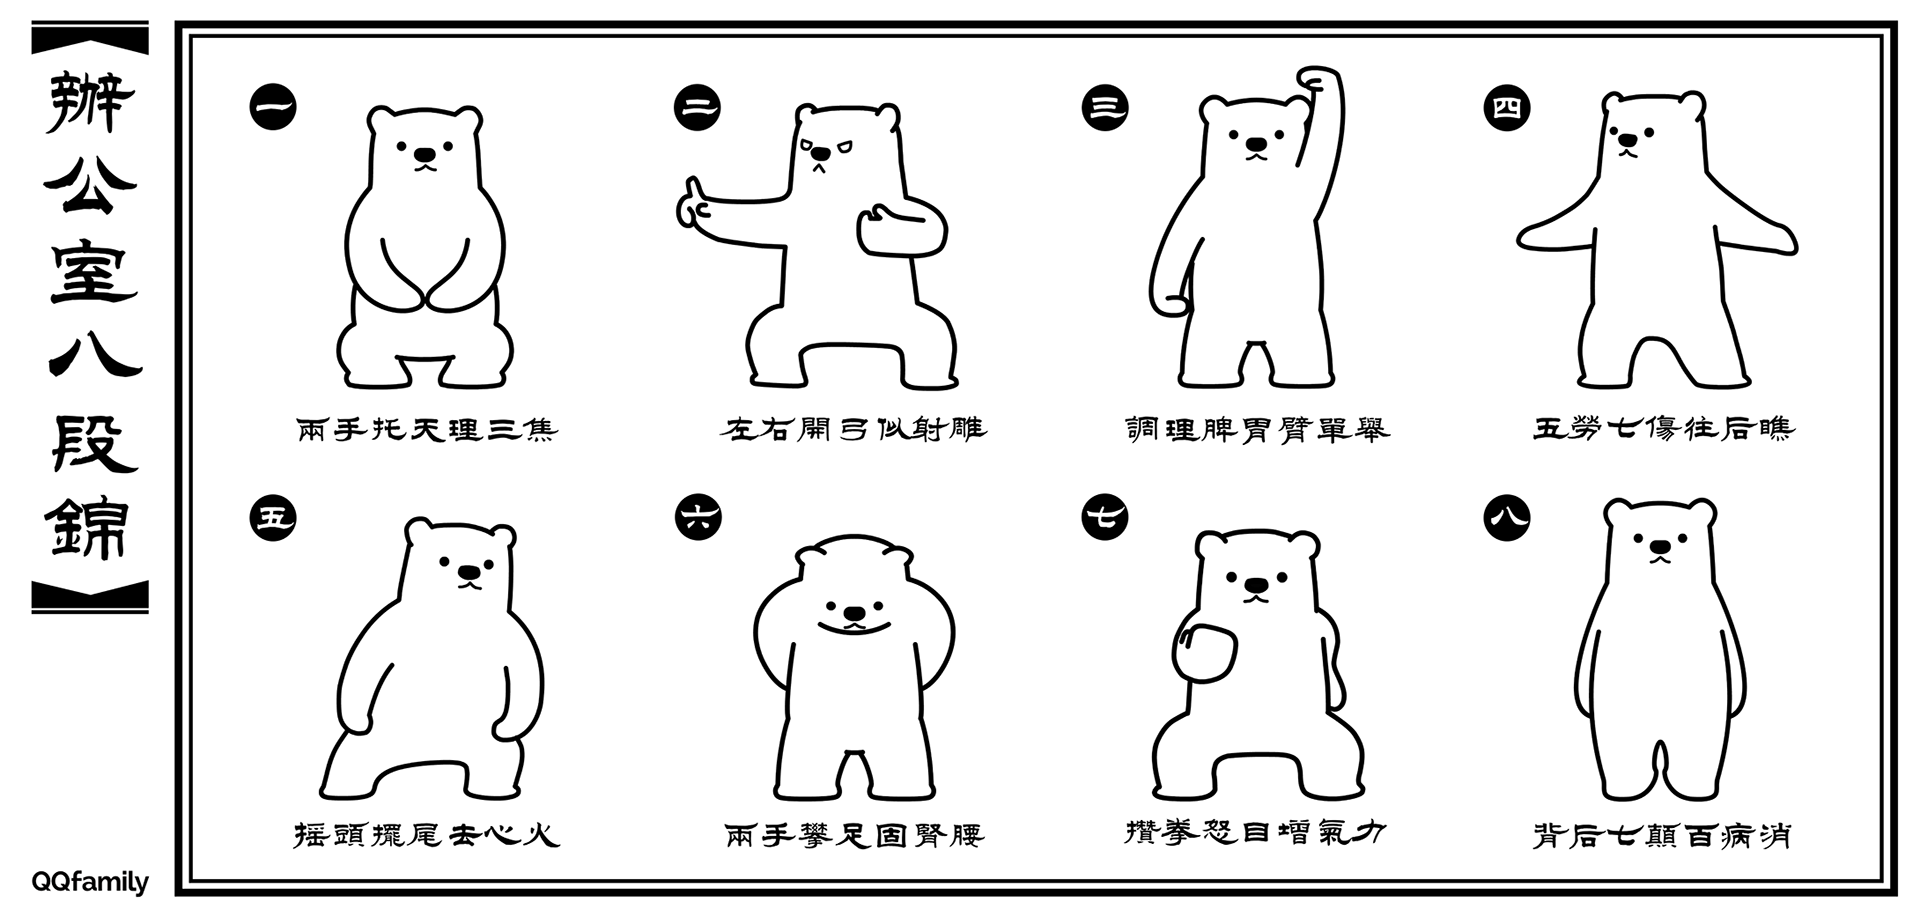
\includegraphics[width=.8\textwidth]{./6ca00034141855.56c56f80ea17f.png}
  \caption{
    QQfamily 办公室八段锦
    \copyright 2015 Tencent. All rights reserved.\cite{QQfamily}
  }
  \label{fig:baduanjin}
\end{figure}

\subsubsection{数据集}

提供的数据集中图像非常不清晰,大多数图像都无法使用 OpenPose 进行手部关键点检测。
图像大小不统一,无法直接送入神经网络。

数据集非常“脏”,有部分图像损坏,甚至每个类别中还都夹杂了并非八段锦的腰鼓表演照片(图 \ref{fig:drum})。

\begin{figure}[h!]
  \centering
  \includegraphics{./baduanjin/data/pose1/pose1_504_9.jpg}
  \caption{训练集中的腰鼓表演图片,文件位于 pose1/pose1\_504\_9.jpg。}
  \label{fig:drum}
\end{figure}

不难发现,数据集中的图像是从视频中按顺序截取的,包含大量连续的动作。若视频中含有多个人,则逐帧裁切其中的所有人物,编号连续。部分图像中照片边缘包含他人四肢,这亦给处理 OpenPose 的生成的 JSON 数据增加了难度。例如,腰鼓的图像(图 \ref{fig:drum})就来自于某段视频的背景,可以看见图片左下方人物。

图像的大小取决于人物的动作:第一、三段的照片中的动作四肢没有向两侧伸展,因此宽高比显著小于其他类别;第二段中上肢水平向侧面伸展,因此其宽高比在所有类别中最大(表 \ref{tab:aspect-ratio})。

\begin{table}[h!]
  \centering
  \begin{tabular}{|l|l|}
    \hline
    段   & 宽高比      \\
    \hline
    第一段 & 0.3781:1 \\
    第二段 & 0.7653:1 \\
    第三段 & 0.4757:1 \\
    第四段 & 0.6435:1 \\
    第五段 & 0.7354:1 \\
    第六段 & 0.6205:1 \\
    第七段 & 0.6244:1 \\
    第八段 & 0.3357:1 \\
    \hline
  \end{tabular}
  \caption{训练集中不同分类图像宽高比的算术平均数。}
  \label{tab:aspect-ratio}
\end{table}

\subsection{项目地址}

\url{https://github.com/wxh06/OpenInnoLab-AI-summer-camp}

\subsection{第一阶段:初步尝试}

\subsubsection{准确率}

训练集:97.84\%;验证集:97.58\%。

\subsubsection{算法}

考虑到图像信息有大量冗余(例如背景),遂使用 MMPose 进行人体姿态估计,提取有效特征。
MMPose 的 \verb|inference_top_down_pose_model| 返回一个包含人物姿态的 17 维特征向量(表 \ref{tab:coco-keypoints})。

\begin{table}[h!]
  \centering
  \begin{tabular}{|r|l|}
    \hline
    Index & Keypoint              \\
    \hline
    0     & \verb|nose|           \\
    1     & \verb|left_eye|       \\
    2     & \verb|right_eye|      \\
    3     & \verb|left_ear|       \\
    4     & \verb|right_ear|      \\
    5     & \verb|left_shoulder|  \\
    6     & \verb|right_shoulder| \\
    7     & \verb|left_elbow|     \\
    8     & \verb|right_elbow|    \\
    9     & \verb|left_wrist|     \\
    10    & \verb|right_wrist|    \\
    11    & \verb|left_hip|       \\
    12    & \verb|right_hip|      \\
    13    & \verb|left_knee|      \\
    14    & \verb|right_knee|     \\
    15    & \verb|left_ankle|     \\
    16    & \verb|right_ankle|    \\
    \hline
  \end{tabular}
  \caption{COCO keypoint indexes \cite{TopDownAicDataset}}
  \label{tab:coco-keypoints}
\end{table}

使用传统机器学习算法来学习特征向量。最基本的 K-近邻算法已经能达到相对不错的性能。
此外,我们还尝试了分类和回归树,其模型准确率略低于 95\%;因此使用了多棵决策树来改进分类性能,最终改用随机森林算法,准确率达到了近 98\%。

\begin{table}[h!]
  \centering
  \begin{tabular}{|l|l|l|}
    \hline
    算法           & 训练准确率   & 验证准确率   \\
    \hline
    KNN          & 95.85\% & 96.30\% \\
    SVM          & 92.68\% & 93.53\% \\
    NaiveBias    & 64.38\% & 63.53\% \\
    CART         & 94.66\% & 94.82\% \\
    AdaBoost     & 63.48\% & 64.23\% \\
    MLP          & 91.33\% & 91.06\% \\
    RandomForest & 97.83\% & 97.58\% \\
    \hline
  \end{tabular}
  \caption{机器学习算法模型性能对比}
  \label{tab:ml-acc}
\end{table}

\subsubsection{模型检验}

然而我们对测试数据进行分类时发现,对于新的数据集,模型的实际准确率粗略估计甚至可能低于 20\%。
笔者推测可能是由于训练集与验证集来自同一数据集,甚至来自于同一视频的连续两帧,特征极为相似,导致模型过拟合较为严重。

\subsection{第二阶段:优化进阶}

\subsubsection{模型}

我们可以构建一个简单的神经网络来代替传统机器学习算法。模型共有三层,为了较快地收敛,前两层的激活函数使用了 ReLU;多分类问题最后一层激活函数应为 softmax,以保证所有选项的概率之和为 1。但经过尝试,性能并不理想,准确率只有 71\%。

\subsubsection{特征提取}

我们注意到 MMPose 的 \verb|inference_top_down_pose_model| 只能估计 17 个关键点,并没有包含可能影响预测结果的四肢尖端的姿态(例如第八段中的踮脚)。
遂决定改用 OpenPose 并进行手部关键点检测。

在 OpenPose 的编译安装过程中遇到了不少麻烦,OpenPose 不兼容较新的 Protocol Buffers 包,而 OpenCV 却依赖于当前版本的 Protobuf;且 Caffe 的 CMake 无法找到苹果 vecLib 库的路径。在尝试了一些变通做法后,最终在 macOS 与 Ubuntu 下都成功编译。
然而手部姿态因图片清晰度问题,有超过半数的图像无法成功标出关键点。此外,OpenPose 生成的关键点坐标数据的单位是像素,在进行训练前需要标准化,处理起来较为麻烦。

很不幸,笔者仅有的 Apple Silicon 以及 AMD Radeon 两块 GPU 均不受 OpenPose 支持,经尝试 CPU 对数据集如此规模的大量数据无能为力。因此最终决定改用 MediaPipe。

MediaPipe 使用的 BlazePose 模型经过优化,能充分利用 CPU 进行运算;且图像中每个人体有 33 个关键点,且每个关键点还包含 z 轴坐标,特征更加丰富。但在检查姿态检测结果时发现有不少图像未能检测到人体,无法送入神经网络进行预测。分析表明,这类图像多见于第六段的弯腰动作,一种变通做法是将所有无法检测到人体的图像全数归为该类。

\subsection{第三阶段:最终实现}

\subsubsection{算法}

笔者最终决定使用卷积神经网络解决分类问题。

正如前文所提到的,数据集每张图像大小不一致,因此在入神经网络之前要进行标准化。将图片大小重设为 $224 \times 224$,再除以 $255.0$ 以保证每一项的数值介于 0 至 1 之间。

模型使用 TensorFlow 2 + Kears 编写。输入是形状为 (None, 224, 224, 3) 的张量;在 DenseNet-121 之后增加一个全连接层,以 softmax 为激活函数;输出是一个形状为 (8,) 的张量,代表每一种分类的概率,所有项之和为 1,对其调用 \verb|tf.argmax| 即可得到最终的预测结果。模型使用分类交叉熵(Categorical Cross Entropy)作为损失函数。

Epoch 被设置为 1,更大的 epochs 会带来过拟合的问题。

实践表明,DenseNet-121 与 ResNet50V2 在这里性能差别不大。

\subsubsection{准确率}

训练集:95.60\%;验证集:99.25\%。

\bibliographystyle{plain}
\bibliography{refs}

\end{document}
